\documentclass[12pt]{article}

\usepackage{sbc-template}

\usepackage{graphicx,url}
\usepackage{booktabs}
\usepackage{multirow}
\usepackage{subfigure}
\usepackage[utf8]{inputenc}
\usepackage{xspace}
\newcommand{\ie}{\emph{i.e.,}\xspace}
\newcommand{\eg}{\emph{e.g.,}\xspace}
\newcommand{\etal}{\emph{et al.}\xspace}
\newcommand{\etc}{\emph{etc.}\xspace}
\sloppy

\title{Assessing pre-training bias in Health data and estimating its impact on machine learning algorithms}

\author{Diego Dimer Rodrigues\inst{1}, Mariana Recamonde-Mendoza\inst{1}}


\address{Instituto de Informática -- Universidade Federal do Rio Grande do Sul
  (UFRGS)\\
  Caixa Postal 15.064 -- 91.501-970 -- Porto Alegre -- RS -- Brazil
  \email{\{ddrodrigues,mrmendoza\}@inf.ufrgs.br}
}

\begin{document} 

\maketitle

\begin{abstract}
  Machine learning (ML) has become a pivotal tool in Health, aiding diagnosis, prognosis, and treatment. However, biases in pre-training data can significantly impact the performance and fairness of ML algorithms. This paper aims to investigate the impact of four pre-training biases in health data and evaluate its effects on three ML models. By leveraging the pre-training metrics on four datasets, we aim to assess the potential for bias and their impact on the models' accuracy. The findings show that more data does not necessarily translate to better performance, highlighting the need to incorporate pre-training bias analysis to ensure fairer models.
\end{abstract}
     
\section{Introduction}
Machine learning (ML) is increasingly used in various domains, including Health, which assists in diagnosis, prognosis, and treatment \cite{Chen2021}. 
However, ML algorithms can potentially introduce biases, leading to unfair and potentially harmful outcomes \cite{obermeyer2019dissecting,juhn2022assessing}. 

This work aims to measure the risk of bias in health datasets using four pre-training bias metrics. It assesses their impact on the performance of supervised ML algorithms and tries to find a correlation between the metric values and the models' performance. The experiments analyze the pre-defined protected attributes from the datasets, assessing the variations in the accuracy score for the protected groups.

\subsection{Class Imbalance (CI)}
CI measures class representation in a dataset, ranging from -1 to 1. Values near zero indicate balance, positive values show an overrepresentation of the advantaged group, and negative values indicate an overrepresentation of the disadvantaged group.

\subsection{Kullback-Leibler (KL) Divergence}
KL Divergence measures the divergence between the label distributions of two facets. It ranges from 0 to $+\infty$, with values near zero indicating similar distributions and higher values indicating more significant divergence.

\subsection{Kolmogorov-Smirnov (KS)}
KS measures the maximum divergence between labels in the distribution for different facets. It ranges from 0 to 1, with values near zero indicating evenly distributed labels and values near one indicating unbalanced labels.

\subsection{Conditional Demographic Disparity in Labels (CDDL)}
CDDL measures the proportion of negative outcomes in a specific facet of a dataset. It ranges from -1 to 1, with positive values indicating demographic disparity favoring the advantaged group and negative values indicating disparity favoring the disadvantaged group.

\section{Related Work}
Many libraries and open-source tools have been developed to address machine learning fairness; for example, the AIF 360 library \cite{Bellamy2018} provides different techniques to identify and mitigate bias. Studies have shown that word embedding algorithms may encode marginalized populations differently, perpetuating social bias. For example, \cite{Zhang2020} demonstrated that such models associated African Americans and Blacks with prison and Whites and Caucasians with hospitals in a fill-in-the-blank style course of action. 
Similarly, Fairness Measures \cite{Zehlike2017} provides different ways of classifying fairness, bias, and discrimination for any \textit{csv} dataset.
Additionally, FairLens \cite{fairlens} is a Python library that automatically discovers and measures bias in data, providing a report on the data quality.

AI models trained on health data can be biased due to protected attributes like ethnicity and race. 
Various studies have explored different approaches for evaluating and mitigating bias in these models. 
\cite {Lopes} analyzed the COMPAS dataset on criminal recidivism and found that the classifier was more prone to predict recidivism for Black people, favoring other demographics. 
In \cite{Noseworthy2020}, the author recommended that AI tools report the model's performance for all the protected attributes.
The study in \cite{Park2021} found that bias mitigation algorithms outperformed simply removing the protected attribute that might cause bias.
\cite{Mandhala2022} used pre-training bias metrics to evaluate bias in models trained on three datasets, finding that mitigation strategies can improve model performance for the unprivileged classes. 

% While numerous works have focused on defining and mitigating bias, we have identified a gap in works that assess the direct impact of pre-training bias on the performance of machine learning algorithms, specifically in the Health domain. In this work, we aim to fill this gap by analyzing the correlation between pre-training bias metrics and the performance of supervised ML algorithms. 

\section{Methodology}
Our methodology involves the following steps:
\begin{enumerate}
    \item Data Collection: We collected four datasets from different sources
    \item Data Preprocessing: We preprocessed the datasets to remove missing values and encode categorical variables
    \item Get Cramer's V Coefficient to find correlated values to the target to calculate CDDL
    \item Increase/Decrease Bias: we artificially tweaked the train sets to introduce or reduce bias, changing data distribution
    \item Train Models: We trained three supervised ML algorithms: Logistic Regression, Decision Tree, and Random Forest, executing 10 splits for each dataset variations
    \item Pre-training Metrics: We calculated the CI, KL Divergence, KS, and CDDL metrics for each dataset, averaging for the ten-fold
    \item Correlation Analysis: We analyzed the correlation between the pre-training bias metrics and the accuracy results of the ML algorithms
\end{enumerate}

The datasets and their source and protected attributes are available in Table~\ref{tab:datasets}. This work uses three supervised learning algorithms: Logistic Regression, Decision Tree, and Random Forest. The models' implementation comes from Python's Scikit-learn library \cite{scikit-learn}, an open-source machine learning library for Python. All hyper-parameters used in training are constant across the four datasets, and all implementations are available in github\footnote{https://github.com/diegodimer/SBCAS2025/}.


\begin{table}[h]
\centering
  \begin{tabular}{@{}rrr@{}}
  \toprule
  Source                                           & Dataset Name              & Protected Attributes        \\ \midrule
  \cite{UCI}                                       & HeartDataset              & Sex                         \\
  \cite{INTERSECTIONAL}                            & IntersectionalBiasDataset & Sex, Race                   \\
  \cite{CDC_Diabetes_Health_Indicators}            & DiabetesDataset           & Sex, Age, Education, Income \\ 
  \cite{Glioma_Grading_Clinical_Mutation_Features} & GliomaDataset             & Gender, Race                \\ \bottomrule
  \end{tabular}
  \caption{Datasets used in this work}
  \label{tab:datasets}
\end{table}
\section{Experiments and Results}

\subsection{Heart Dataset}
\label{sec:heart}
The first dataset was the Heart dataset, a real-life scenario collected from patients, consisting of around 300 instances, used to predict heart disease. The performance for each dataset variation and the mean dataset size used for the training are in Table~\ref{tab:acc-heart}.

For the \textbf{highly unbalanced} version of this dataset, we removed 85\% of women with thal equals 2 and negative output, 80\% of women with thal equals 3 and negative output, 80\% of women with cp equals 2 and negative output, 80\% of women with cp equals 0 and negative output, and 20\% of instances with positive output. These changes resulted in increasing the values for all metrics. However, CDDL was still above 0.4 for the two correlated variables. In the \textbf{equally balanced} version, we managed to get all metrics close to zero. The complete report of the metrics is in Table~\ref{tab:metrics-health}. 

The results do not indicate the impact of the pre-training metrics, as seen in Figure~\ref{fig:relative-health}, since false positive and false negative rates were similar across dataset variations. Feature importance analysis, shown in Figure~\ref{fig:importances-health}, suggests that the varying attributes may not have significantly influenced the decision-making process.

\begin{figure}[ht]
\centering
    \subfigure[Original]
    {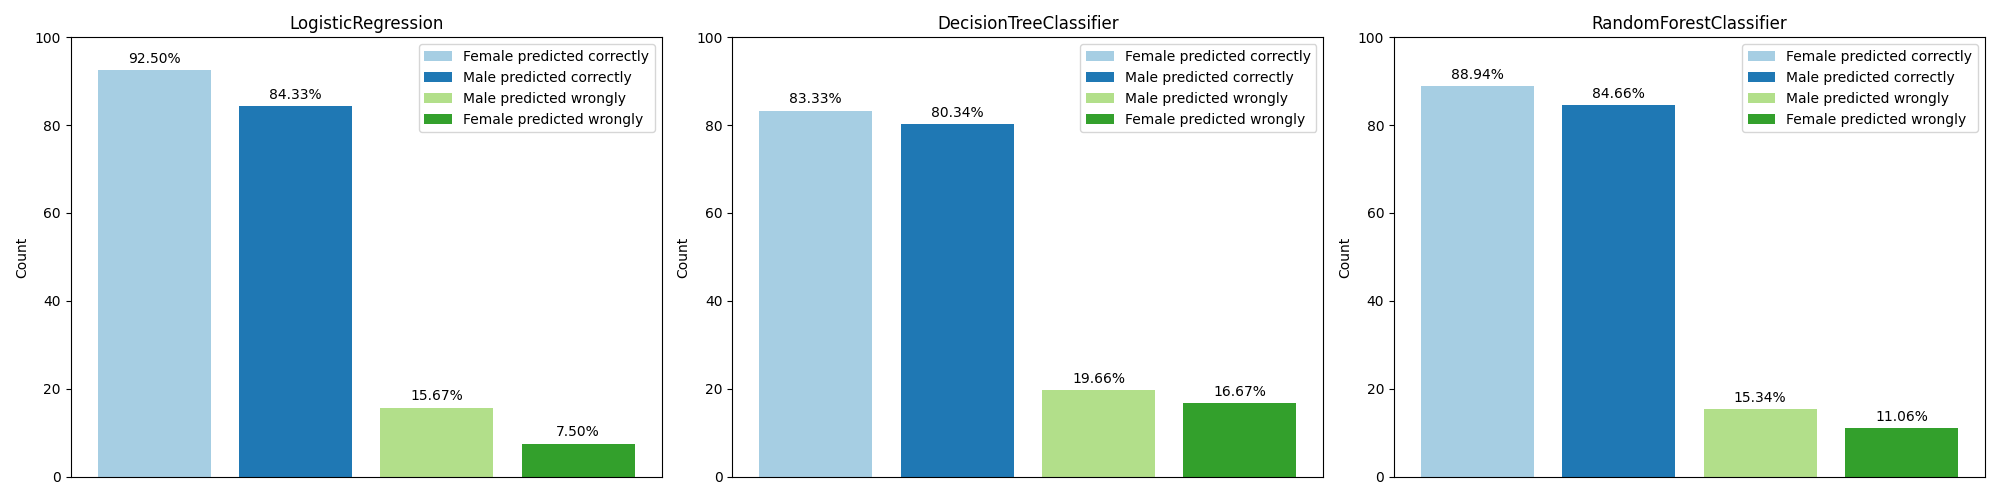
\includegraphics[width=.8\textwidth]{results/HeartDataset/original-dataset/barchart-relative-sex.png}
    \label{fig:original-relative-health}}  
    \subfigure[Highly unbalanced]
    {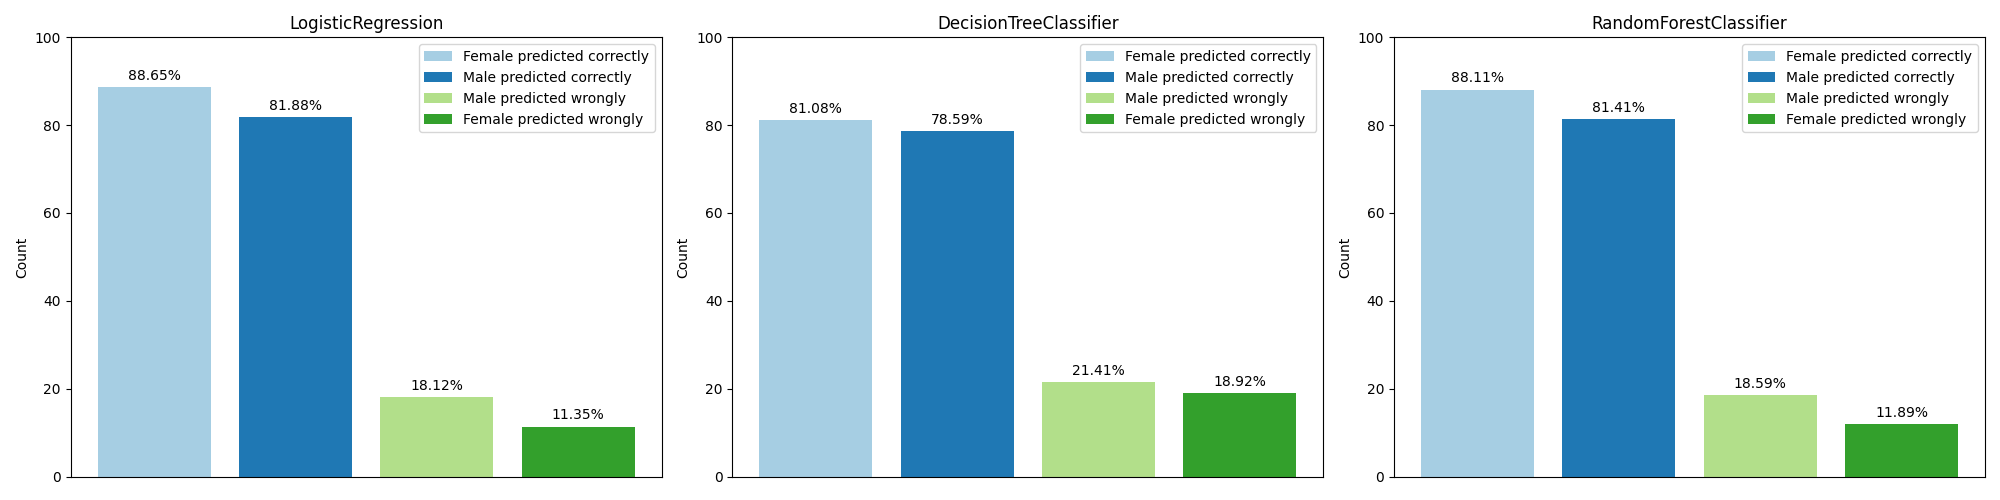
\includegraphics[width=.8\textwidth]{results/HeartDataset/high-imbalance/barchart-relative-sex.png} \label{fig:high-relative-health}} 
        \hfil
    \subfigure[Equally balanced]
    {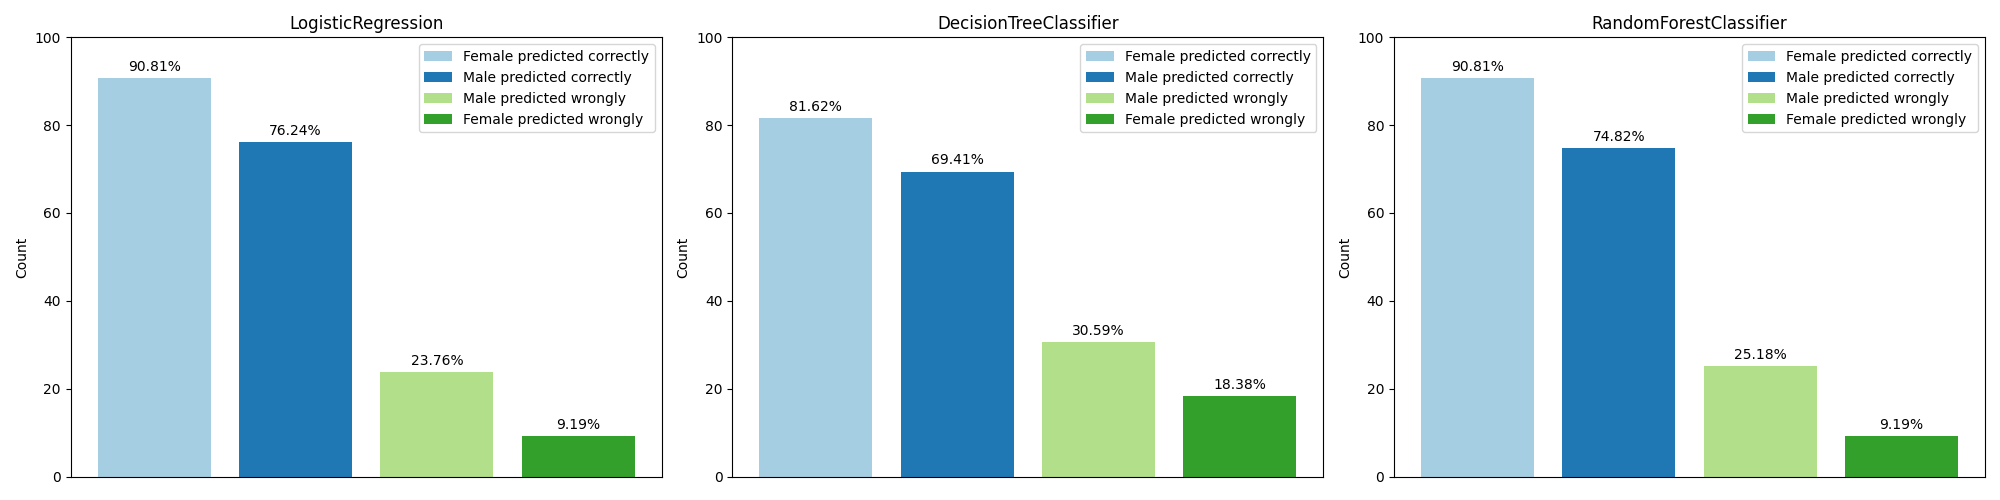
\includegraphics[width=.8\textwidth]{results/HeartDataset/equal-balance/barchart-relative-sex.png} \label{fig:equal-relative-health}} 
    \caption{Prediction results for the feature sex on the Health dataset.}
    \label{fig:relative-health}
\end{figure}




\begin{table}[ht]
\centering
\begin{tabular}{@{}rrrr@{}}
\toprule
                      & Original & High Imbalance & Equal Balance \\ \midrule
Class Imbalance (sex) & 0.357    & 0.548          & 0.000         \\
KL Divergence (sex)   & 0.202    & 1.346          & 0.000         \\
KS (sex)              & 0.299    & 0.524          & 0.000         \\
CDDL (sex, cp)        & 0.291    & 0.375          & 0.086         \\
CDDL (sex, thal)      & 0.108    & 0.275          & -0.123        \\ \bottomrule
\end{tabular}
\caption{Pre-training metrics for the Health dataset}
\label{tab:metrics-health}
\end{table}


\begin{table}[ht]
  \centering
  \begin{tabular}{@{}rrrrr@{}}
  \toprule
                                    & Attribute            & Class  & Accuracy  & Mean Train Set Size    \\ \midrule
  \multirow{2}{*}{Original Dataset} & \multirow{2}{*}{Sex} & Female & 86.486 & \multirow{2}{*}{241.0} \\
                                    &                      & Male   & 79.608 &                        \\ \midrule
  \multirow{2}{*}{High Imbalance}   & \multirow{2}{*}{Sex} & Female & 85.946 & \multirow{2}{*}{211.2} \\
                                    &                      & Male   & 80.627 &                        \\ \midrule
  \multirow{2}{*}{Equal Balance}    & \multirow{2}{*}{Sex} & Female & 87.748 & \multirow{2}{*}{155.0} \\
                                    &                      & Male   & 73.490 &                        \\ \bottomrule
  \end{tabular}
  \caption{Accuracy results on the protected attributes for the Heart dataset}
  \label{tab:acc-heart}
\end{table}


\subsection{Intersectional-bias Dataset}
\label{sec:intersectional}
The second dataset is an artificial dataset created to predict a diagnosis (of schizophrenia or depression). The dataset contained two protected attributes, sex (with "female" as the unprivileged class) and race (with "non-white" as the unprivileged class); the performance in the protected attribute is reported in Table~\ref{tab:acc-intersectional}. We do identify that the performance, especially in the Sex attribute, was affected in the highly unbalanced version, with "female" having close to 9\% less accuracy; however, this could also be caused by the number of instances in the train set size since the equally balanced that had better performance was more than 2 times larger, and the original was even larger. 

To achieve the metrics' values reported in Table~\ref{tab:metrics-intersectional}, in the \textbf{high imbalance} version, we remove 95\% of instances of non-white with negative output, 50\% of non-white with positive output, 80\% of women with negative output, and 95\% of women with positive output. It is also noted that the metrics for the sex attribute did not get above 0.5; increasing them would lead to even less data in the training set, deviating from the metrics' analysis.

% \begin{figure}[ht]
%     \centering
%         \subfigure[Original]
%         {\includegraphics[width=.8\textwidth]{results/IntersectionalBiasDataset/original-dataset/barchart-relative-race.png}
%         \label{fig:original-relative-intersectional}}  
%         \subfigure[Highly unbalanced]
%         {\includegraphics[width=.8\textwidth]{results/IntersectionalBiasDataset/high-imbalance/barchart-relative-race.png} \label{fig:high-relative-intersectional}} 
%             \hfil
%         \subfigure[Equally balanced]
%         {\includegraphics[width=.8\textwidth]{results/IntersectionalBiasDataset/equal-balance/barchart-relative-race.png} \label{fig:equal-relative-intersectional}} 
%         \caption{Prediction results for the feature Race on the Intersectional Bias dataset.}
%         \label{fig:relative-health}
% \end{figure}

% \begin{figure}[ht]
%     \centering
%         \subfigure[Original]
%         {
\includegraphics[width=.8\textwidth]{results/IntersectionalBiasDataset/original-dataset/barchart-relative-sex.png}
%         \label{fig:original-relative-intersectional}}  
%         \subfigure[Highly unbalanced]
%         {
\includegraphics[width=.8\textwidth]{results/IntersectionalBiasDataset/high-imbalance/barchart-relative-sex.png} \label{fig:high-relative-intersectional}} 
%             \hfil
%         \subfigure[Equally balanced]
%         {
\includegraphics[width=.8\textwidth]{results/IntersectionalBiasDataset/equal-balance/barchart-relative-sex.png} \label{fig:equal-relative-intersectional}} 
%         \caption{Prediction results for the feature Sex on the Intersectional Bias dataset.}
%         \label{fig:relative-health}
% \end{figure}

\begin{figure}[ht]
    \centering
    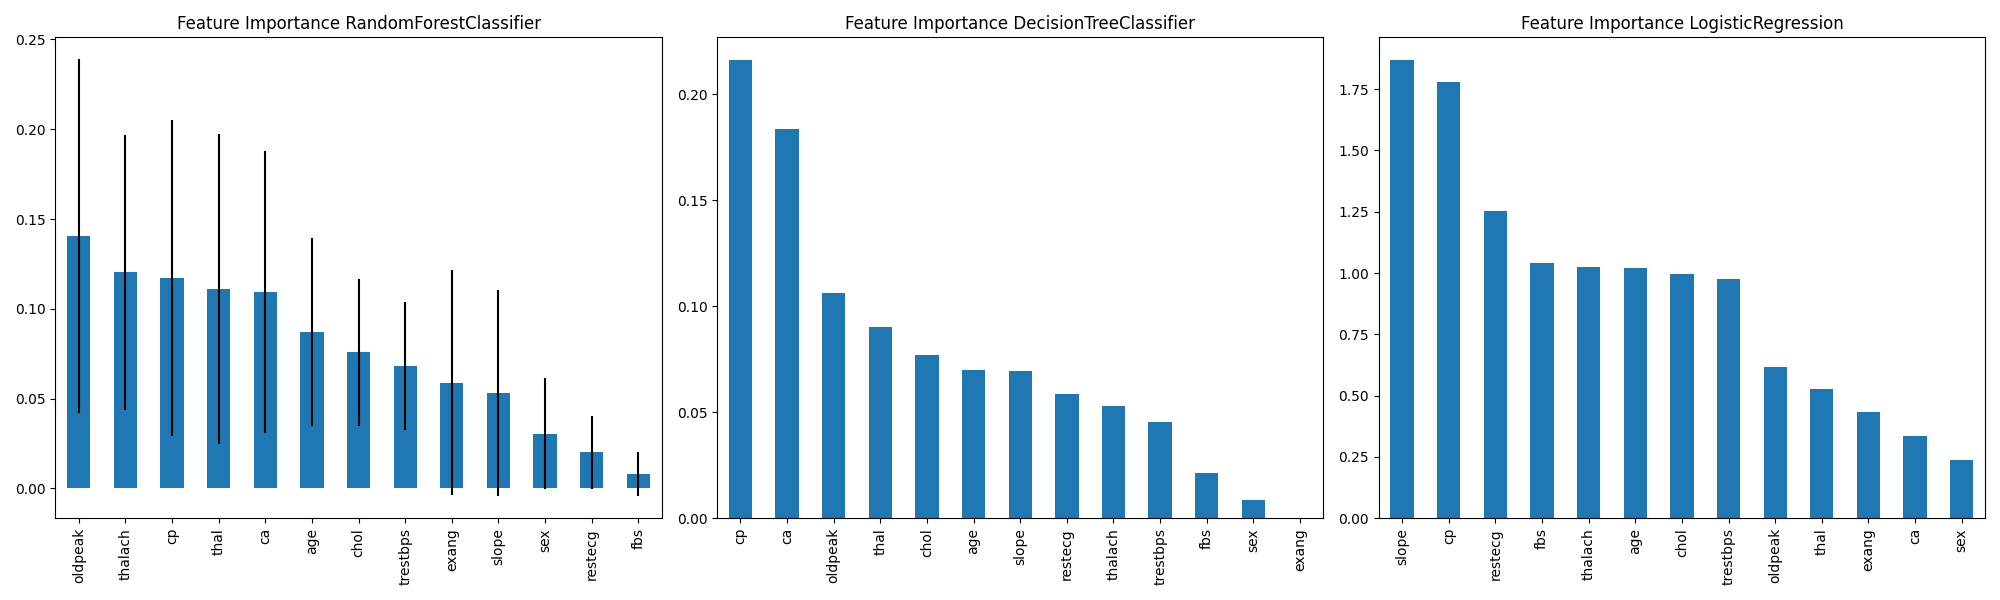
\includegraphics[width=0.9\linewidth]{results/HeartDataset/original-dataset/importances.png}
    \caption{Feature Importance for the original version of the Health dataset}
    \label{fig:importances-health}
\end{figure}

\begin{table}[ht]
\centering
\begin{tabular}{@{}rrrr@{}}
\toprule
                        & Original & High Imbalance & Equal Balance \\ \midrule
Class Imbalance (Sex)   & -0.103   & 0.755          & 0.000         \\
KL Divergence (Sex)     & 0.077    & 0.474          & 0.000         \\
KS (Sex)                & 0.195    & 0.459          & 0.000         \\
CDDL (Sex, Rumination)  & -0.184   & -0.207         & 0.005         \\
Class Imbalance (Race)  & -0.268   & 0.235          & 0.000         \\
KL Divergence (Race)    & 0.018    & 0.938          & 0.000         \\
KS (Race)               & 0.096    & 0.503          & 0.000         \\
CDDL (Race, Rumination) & 0.079    & 0.500          & -0.007        \\ \bottomrule
\end{tabular}
\caption{Pre-training metrics for the Intersectional bias dataset}
\label{tab:metrics-intersectional}
\end{table}

\begin{table}[ht]
  \centering
  \begin{tabular}{@{}rrrrr@{}}
  \toprule
                                    & Attribute             & Class     & Accuracy  & Mean Train Set Size     \\ \midrule
  \multirow{4}{*}{Original Dataset} & \multirow{2}{*}{Sex}  & Female    & 80.994 & \multirow{4}{*}{5280.0} \\
                                    &                       & Male      & 95.207 &                         \\
                                    & \multirow{2}{*}{Race} & Non-White & 85.849 &                         \\
                                    &                       & White     & 90.090 &                         \\ \midrule
  \multirow{4}{*}{High Imbalance}   & \multirow{2}{*}{Sex}  & Female    & 71.423 & \multirow{4}{*}{1529.7} \\
                                    &                       & Male      & 93.594 &                         \\
                                    & \multirow{2}{*}{Race} & Non-White & 77.317 &                         \\
                                    &                       & White     & 88.512 &                         \\ \midrule
  \multirow{4}{*}{Equal Balance}    & \multirow{2}{*}{Sex}  & Female    & 79.932 & \multirow{4}{*}{3114.4} \\
                                    &                       & Male      & 94.317 &                         \\
                                    & \multirow{2}{*}{Race} & Non-White & 83.927 &                         \\
                                    &                       & White     & 90.723 &                         \\ \bottomrule
  \end{tabular}
  \caption{Accuracy results on the protected attributes for the Intersectional Bias dataset}
  \label{tab:acc-intersectional}
\end{table}



\subsection{Glioma Dataset}
\label{sec:glioma}
The Glioma dataset contains information about 20 genes (mutated or not) for the classification of brain tumors that can be classified into LGG (Lower-Grade Glioma) or GBM (Glioblastoma Multiforme). This dataset also contains two protected attributes: Gender (with "female" being the unprivileged) and Race (with "non-white" being the unprivileged). To make the \textbf{highly unbalanced} version on this dataset, we removed 70\% of women with Grade 1, 75\% of men with Grade 0, 75\% of non-white people with Grade 0, and 55\% of white people with Grade 1, respectively. This dataset's complete metrics' values are in Table~\ref{tab:metrics-glioma}. 

In this dataset, we observed a different pattern: the highly unbalanced version had the worst performance compared to the other two, with around three times more data than the equally balanced version, and the performance affected primarily females and non-white people, as reported in Table~\ref{tab:acc-glioma}. As we see in Figure~\ref{fig:relative-glioma}, especially in \ref{fig:high-relative-glioma}, we can infer that all models were prone to wrongly predict negative for women, which would result in misdiagnosing for specific groups. The importance of each variable for the particular models, as reported in Figure~\ref{fig:importances-glioma}, does not show the protected attributes as important features and shows \textit{Age\_at\_diagnosis} (which is correlated to the protected attributes) as important to the decision-making process in the decision trees.  

\begin{figure}[ht] % talvez deixar só o gráfico do high imbalance?
    \centering
        \subfigure[Original]
        {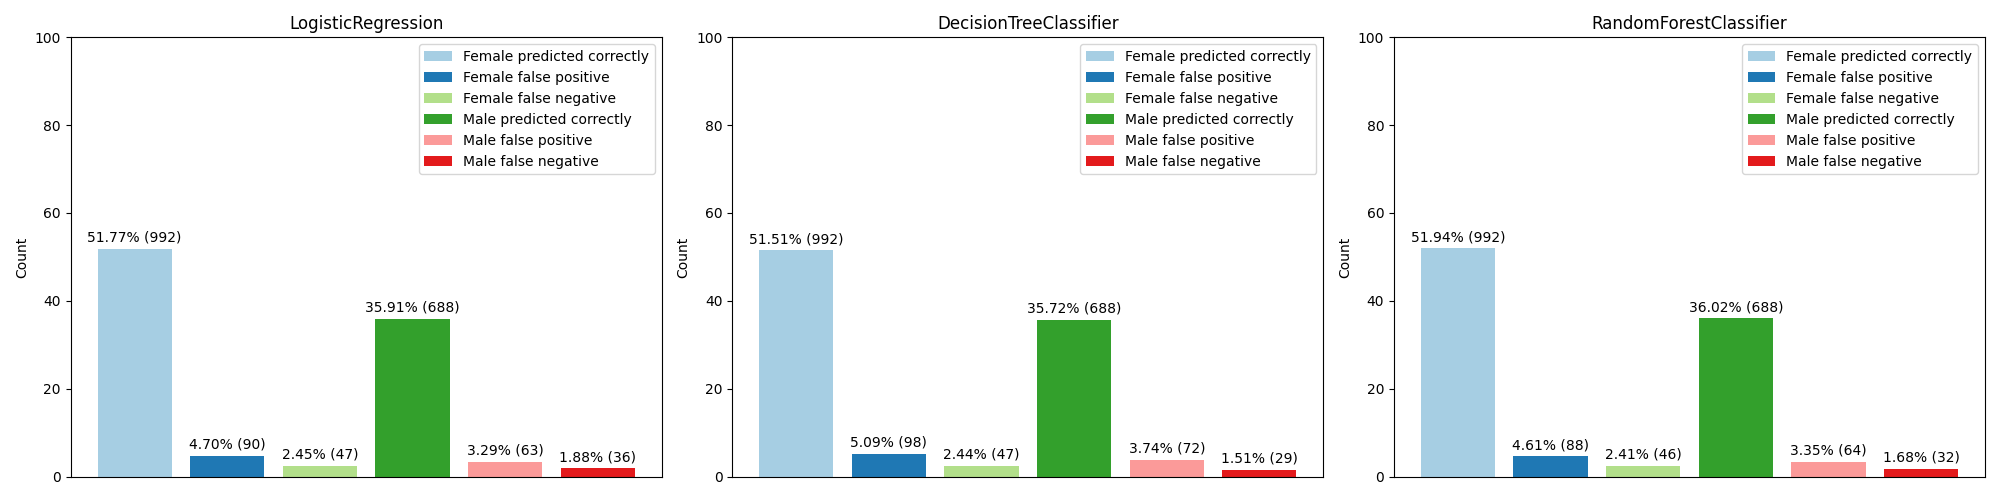
\includegraphics[width=1\textwidth]{results/GliomaDataset/original-dataset/barchart-complete-Gender.png}
        \label{fig:original-relative-glioma}}  
        \subfigure[Highly unbalanced]
        {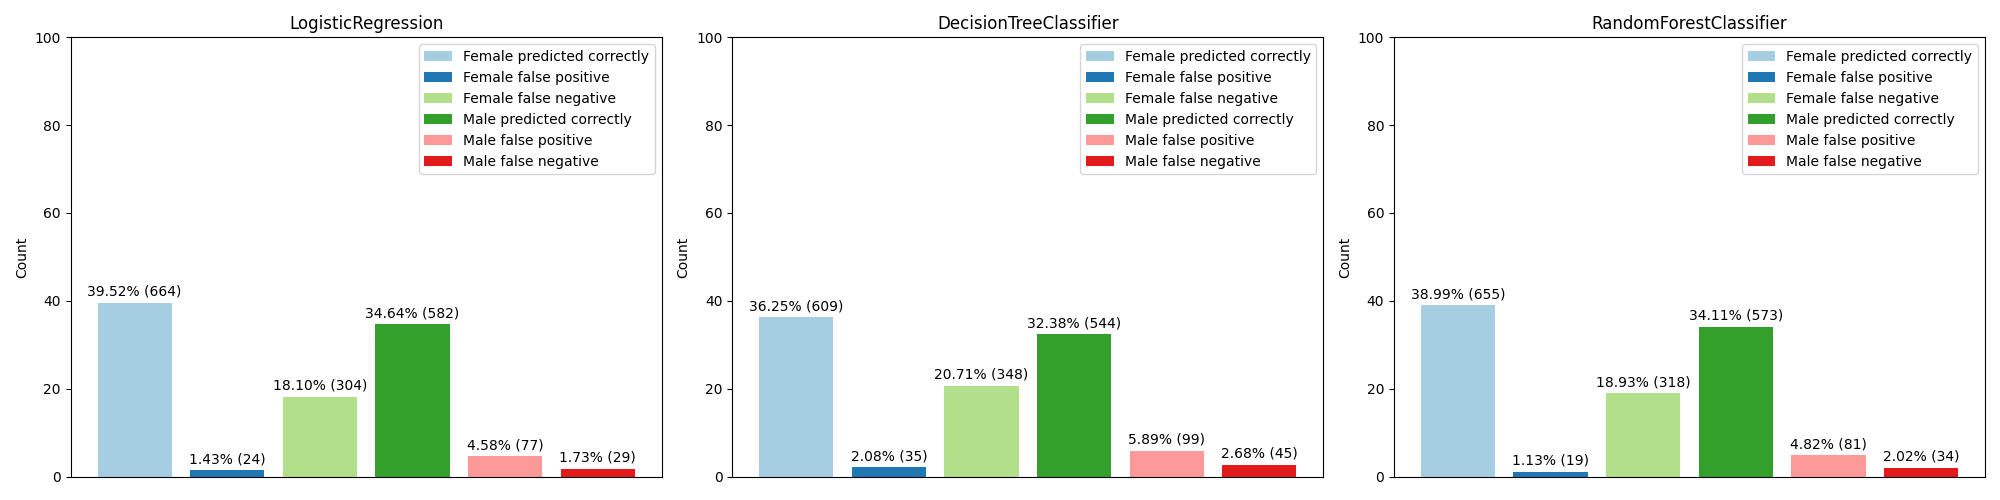
\includegraphics[width=1\textwidth]{results/GliomaDataset/high-imbalance/barchart-complete-Gender.png} \label{fig:high-relative-glioma}} 
            \hfil
        \subfigure[Equally balanced]
        {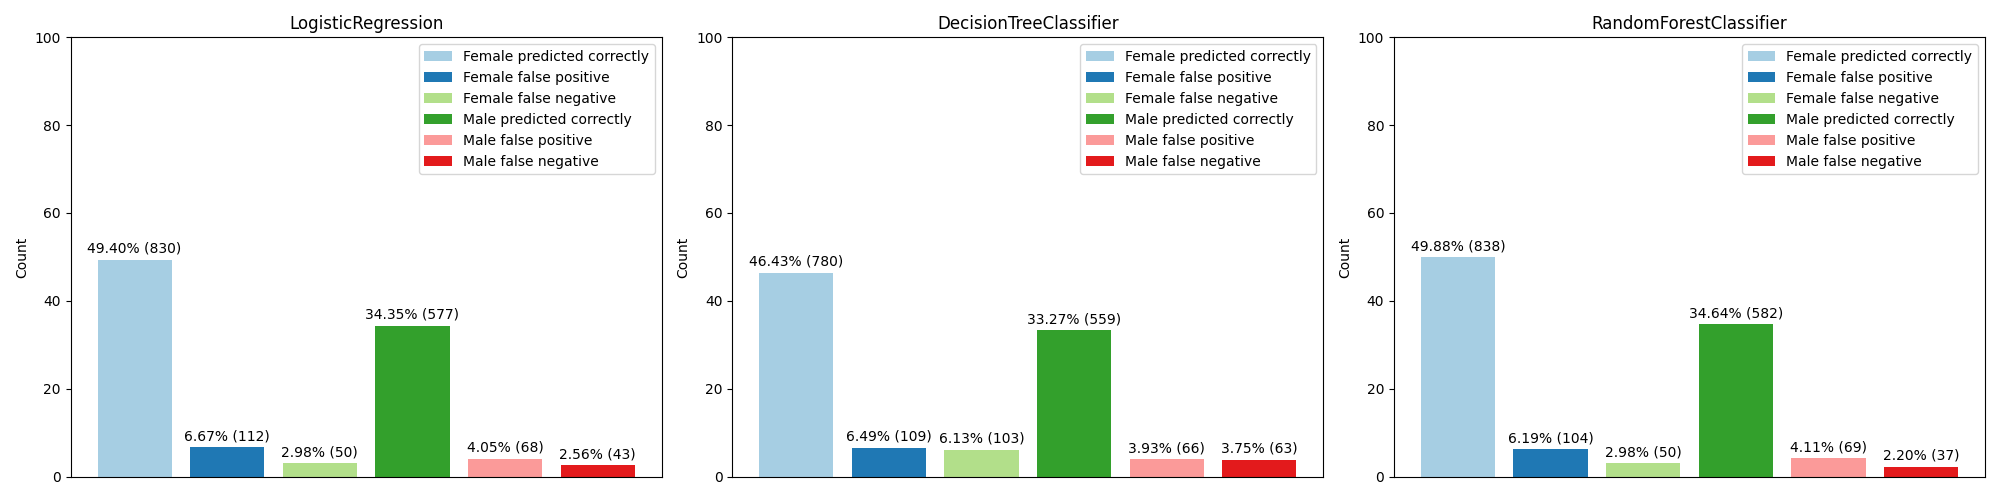
\includegraphics[width=1\textwidth]{results/GliomaDataset/equal-balance/barchart-complete-Gender.png} \label{fig:equal-relative-glioma}} 
        \caption{Prediction results for the feature Gender on the Glioma dataset.}
        \label{fig:relative-glioma}
\end{figure}

\begin{table}[ht]
\centering
\begin{tabular}{@{}rrrr@{}}
\toprule
                                  & Original & High Imbalance & Equal Balance \\ \midrule
Class Imbalance (Gender)          & -0.158   & -0.415         & -0.197        \\
KL Divergence (Gender)            & 0.008    & 0.601          & 0.028         \\
KS (Gender)                       & 0.062    & 0.454          & 0.118         \\
CDDL (Gender, Age\_at\_diagnosis) & -0.061   & -0.535         & 0.064         \\
Class Imbalance (Race)            & 0.822    & 0.857          & -0.032        \\
KL Divergence (Race)              & 0.080    & 0.994          & 0.000         \\
KS (Race)                         & 0.199    & 0.638          & 0.000         \\
CDDL (Race, Age\_at\_diagnosis)   & 0.021    & 0.054          & 0.001         \\ \bottomrule
\end{tabular}
\caption{Pre-training metrics for the Glioma dataset}
\label{tab:metrics-glioma}
\end{table}

\begin{table}[ht]
  \centering
  \begin{tabular}{@{}rrrrr@{}}
  \toprule
                                    & Attribute               & Class     & Accuracy  & Mean Train Set Size    \\ \midrule
  \multirow{4}{*}{Original Dataset} & \multirow{2}{*}{Gender} & Female    & 86.022 & \multirow{4}{*}{670.0} \\
                                    &                         & Male      & 85.659 &                        \\
                                    & \multirow{2}{*}{Race}   & Non-White & 74.537 &                        \\
                                    &                         & White     & 86.936 &                        \\ \midrule
  \multirow{4}{*}{High Imbalance}   & \multirow{2}{*}{Gender} & Female    & 64.785 & \multirow{4}{*}{332.0} \\
                                    &                         & Male      & 82.316 &                        \\
                                    & \multirow{2}{*}{Race}   & Non-White & 66.204 &                        \\
                                    &                         & White     & 72.504 &                        \\ \midrule
  \multirow{4}{*}{Equal Balance}    & \multirow{2}{*}{Gender} & Female    & 82.258 & \multirow{4}{*}{93.4}  \\
                                    &                         & Male      & 83.236 &                        \\
                                    & \multirow{2}{*}{Race}   & Non-White & 67.824 &                        \\
                                    &                         & White     & 84.049 &                        \\ \bottomrule
  \end{tabular}
  \caption{Accuracy results on the protected attributes for the Glioma dataset}
  \label{tab:acc-glioma}
\end{table}

\begin{figure}[ht]
    \centering
    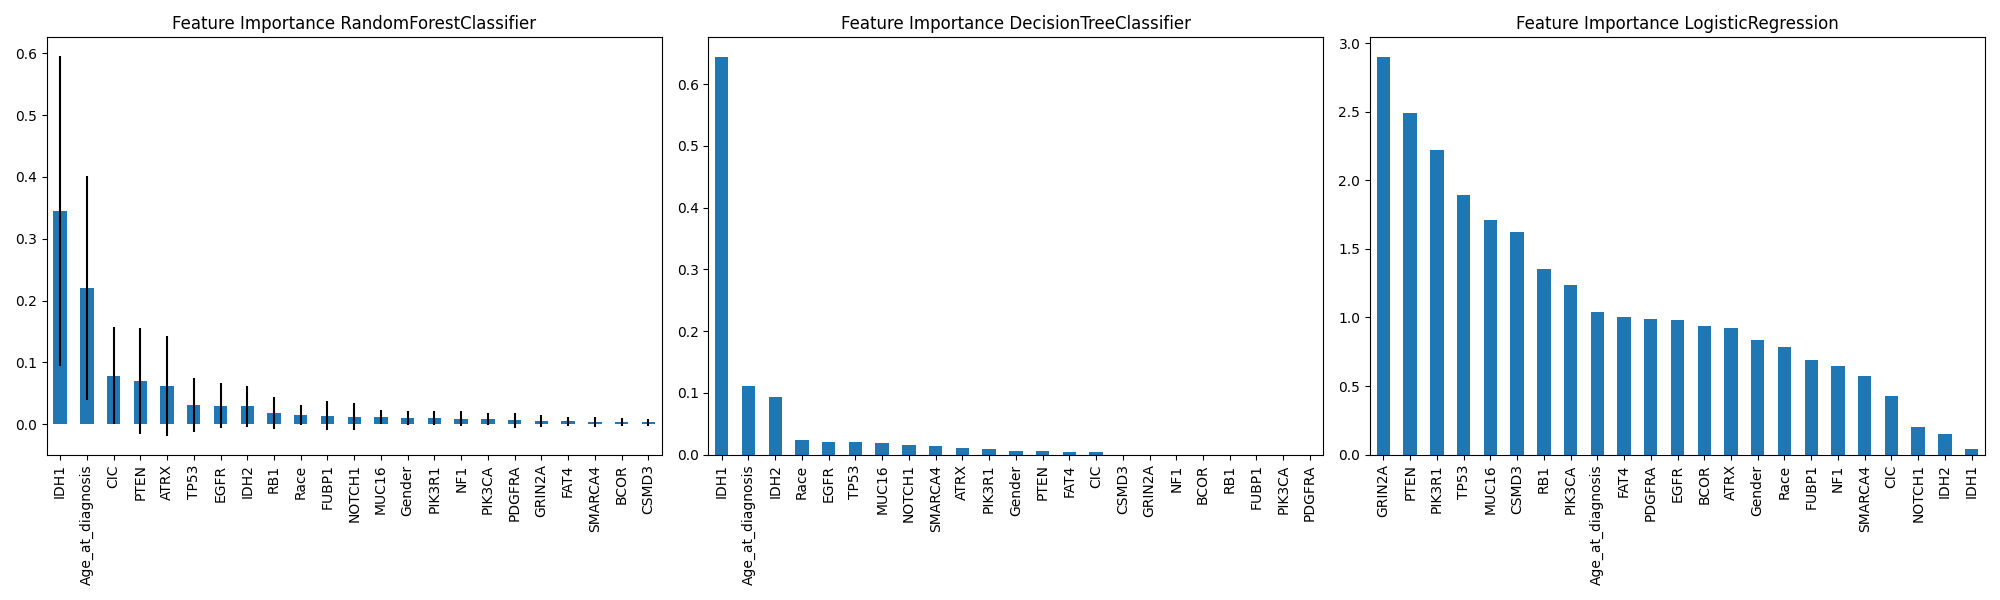
\includegraphics[width=0.8\linewidth]{results/GliomaDataset/original-dataset/importances.png}
    \caption{Feature Importance for the original version of the Glioma dataset}
    \label{fig:importances-glioma}
\end{figure}


\subsection{Diabetes Dataset}
\label{sec:diabetes}
The diabetes dataset contains 70,692 survey responses. The target variable Diabetes\_binary has 2 classes: 0 is for no diabetes, and 1 is for prediabetes or diabetes. This dataset has 21 features, and for the experiments, we considered Sex and Age for the analysis of pre-training bias. The accuracy results for the two protected attributes are in Table~\ref{tab:acc-diabetes}.

In the \textbf{highly unbalanced} version of this dataset, we removed 85\% of women with negative output, 85\% of men with positive output, 55\% of people aged between 18 and 24 with positive output, 45\% of people with age above 24 with negative output, 20\% of women with low blood pressure with negative output and 20\% of men with high blood pressure with positive output, respectively. The report on the metrics' values is in Table~\ref{tab:metrics-diabetes}.

In this dataset, we see that the high values from the metrics do translate to the performance on the unprivileged classes, especially for females, with an accuracy 30\% lower than the other variations, even with the highly imbalanced dataset containing 53 times more data than the equally balanced. In the age attribute, the opposite occurred; accuracy was lower in the privileged class (age above 24). Analyzing the importance of each feature for this dataset, as shown in Figure~\ref{fig:importances-diabetes}, we can see that protected attributes were not the most important features in the decision-making process, but the unbalance of these attributes reflected directly in the performance for the unprivileged groups.

\begin{table}[ht]
\centering
\begin{tabular}{@{}rrrr@{}}
\toprule
                      & Original & High Imbalance & Equal Balance \\ \midrule
Class Imbalance (Sex) & -0.122   & 0.247          & 0.000         \\
KL Divergence (Sex)   & 0.002    & 1.064          & 0.000         \\
KS (Sex)              & 0.024    & 0.681          & 0.003         \\
CDDL (Sex, HighBP)    & -0.044   & 0.744          & -0.005        \\
Class Imbalance (Age) & 0.952    & 0.905          & 0.000         \\
KL Divergence (Age)   & 0.241    & 0.900          & 0.159         \\
KS (Age)              & 0.142    & 0.314          & 0.136         \\
CDDL (Age, HighBP)    & -0.022   & -0.057         & -0.397        \\ \bottomrule
\end{tabular}
\caption{Pre-training metrics for the Diabetes dataset}
\label{tab:metrics-diabetes}
\end{table}

\begin{table}[ht]
  \centering
  \begin{tabular}{@{}rrrrr@{}}
  \toprule
                                    & Attribute            & Class      & Accuracy  & Mean Train Set Size       \\ \midrule
  \multirow{4}{*}{Original Dataset} & \multirow{2}{*}{Sex} & Female     & 86.205 & \multirow{4}{*}{183579.0} \\
                                    &                      & Male       & 83.719 &                           \\
                                    & \multirow{2}{*}{Age} & Unprileged & 83.245 &                           \\
                                    &                      & Privileged & 85.120 &                           \\ \midrule
  \multirow{4}{*}{High Imbalance}   & \multirow{2}{*}{Sex} & Female     & 53.063 & \multirow{4}{*}{53216.9}  \\
                                    &                      & Male       & 83.352 &                           \\
                                    & \multirow{2}{*}{Age} & Unprileged & 70.975 &                           \\
                                    &                      & Privileged & 66.299 &                           \\ \midrule
  \multirow{4}{*}{Equal Balance}    & \multirow{2}{*}{Sex} & Female     & 84.570 & \multirow{4}{*}{1002.4}   \\
                                    &                      & Male       & 82.276 &                           \\
                                    & \multirow{2}{*}{Age} & Unprileged & 80.790 &                           \\
                                    &                      & Privileged & 83.575 &                           \\ \bottomrule
  \end{tabular}
  \caption{Accuracy results on the protected attributes for the Diabetes dataset}
  \label{tab:acc-diabetes}
  \end{table}

\begin{figure}[ht]
    \centering
    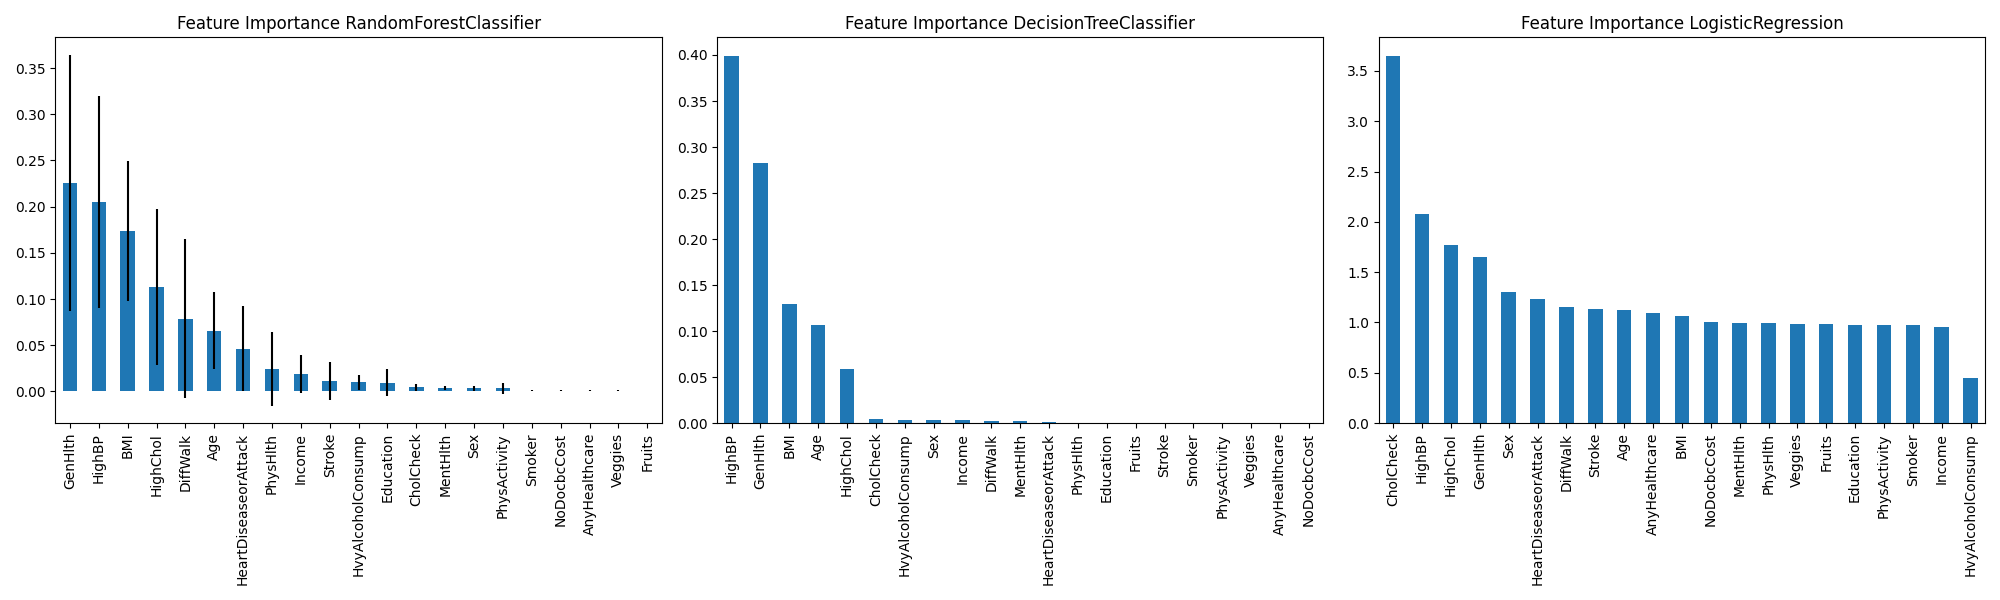
\includegraphics[width=0.9\linewidth]{results/DiabetesDataset/original-dataset/importances.png}
    \caption{Feature Importance for the original version of the Diabetes dataset}
    \label{fig:importances-diabetes}
\end{figure}

\section{General Discussion}

Based on the results from the four analyzed datasets, we can discuss the impact of pre-training metrics and their influence on model performance across the three different models we trained. Specifically, the findings presented in sections~\ref{sec:diabetes} and~\ref{sec:glioma} suggest that when our dataset increases without considering the implications for model fairness, we increase the risk of accumulating biased data that may result in decreased accuracy in our results, particularly affecting historically underrepresented groups. It's also important to note that the results are consistent across all three trained models, indicating that the bias impacted the models equally, regardless of the algorithm used. 

Analysis of feature importance in the different dataset variations shows that for all datasets except the Heart Dataset (discussed in Section~\ref{sec:heart}), the highly unbalanced versions considered the protected features important to the model predictions (among the five more important features); this is especially true for the tree-based models (decision tree and random forest).

The complete set of charts, tables, code, and instructions on reproducing the experiments presented in this work are available on github\footnote{https://github.com/diegodimer/SBCAS2025}.

\section{Conclusion}

In this work, we assessed the impact of pre-training bias on the performance of machine learning algorithms in health datasets. We analyzed four pre-training bias metrics: Class Imbalance (CI), Kullback-Leibler (KL) Divergence, Kolmogorov-Smirnov (KS), and Conditional Demographic Disparity in Labels (CDDL). Our experiments on four datasets demonstrated that high values of these metrics often correlate with decreased performance for unprivileged groups, especially in the last two datasets (Glioma and Diabetes) we observed that the train set size might not be associated with the performance, as the highly imbalanced dataset had more data than the equally balanced version and reported worse performance. We also note that the pre-training metrics had a more significant impact on the datasets with more data, and real-life scenarios seemed to incorporate more bias than artificial datasets (as seen in the IntersectionalBias dataset).

We highlight the need to address bias before training models, as the pre-training metrics can give some insights into the quality of the models trained before spending any computational resources.

Future work includes the following: analyzing the complete set of features on the dataset to generalize bias investigation beyond the protected attributes; conducting sensibility analysis for the metrics values to better measure the risk of bias from a numeric perspective; incorporating model explainability techniques such as PCA and SHAP values to explain the classifiers biased predictions; incorporating new performance metrics and strategies to mitigate the bias and their effects on the pre-training metrics.



\clearpage 
%\section{References}

\bibliographystyle{sbc}
\bibliography{sbc-template}

\end{document}
